
Please insert your deliverables for Stage4 as follows:
\begin{itemize} 
\item{Unzip the interface web page and related data into a directory, run the command "python -m SimpleHTTPServer 8000" (if using python 2) or "python -m http.server 8000"(if using python 3) in the directory, then use a web browser and navigate to localhost: 8000/ house data filter.html. The initial screen shot:
\begin{figure}
\centering
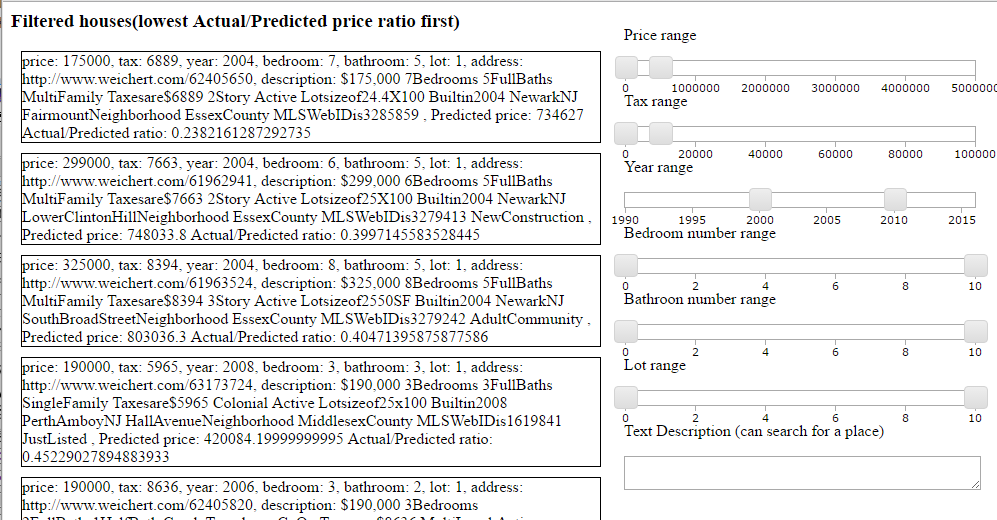
\includegraphics[width=0.5\textwidth]{houseinitial.png}
\caption{}
\end{figure}

	
\item{Two different  sample navigation user paths through the data exemplifying the different modes of interaction and the corresponding screen shots. 

1. The user wants to find cheap small houses, so slide the bedroom, bathroom, price and tax sliders to the left, then the web page will display the houses that seem like deals according to the actual price to predicted price ratio. The predicted price is calculated with the coefficients obtained from linear regression.

\i\begin{figure}
\centering
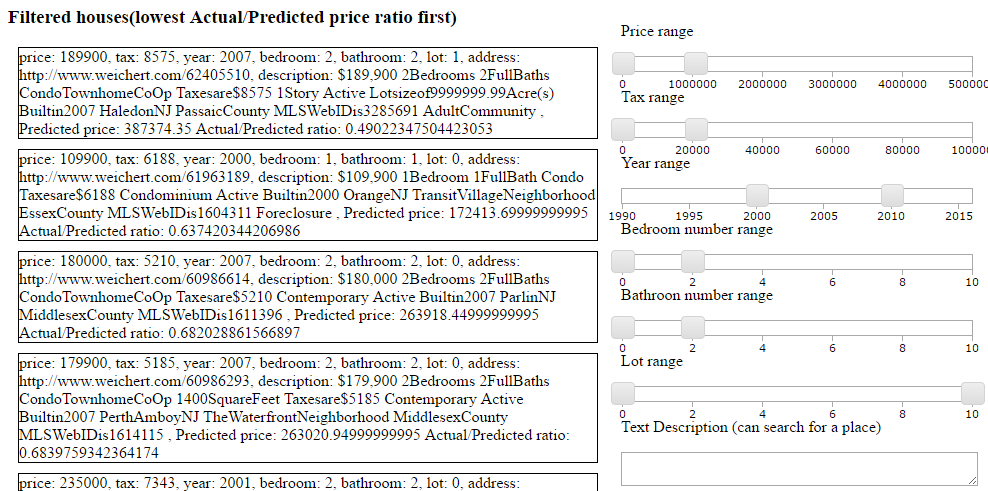
\includegraphics[width=0.5\textwidth]{housesmall.png}
\caption{}
\end{figure}

2. The user wants to find any houses that are deals in the Edison region, so type the text "Edison" (case sensitive) into the Text description search box, and slide all sliders as wide apart as possible. The top houses displayed are the ones that seem to be deals according to the linear regression.

\begin{figure}
\centering
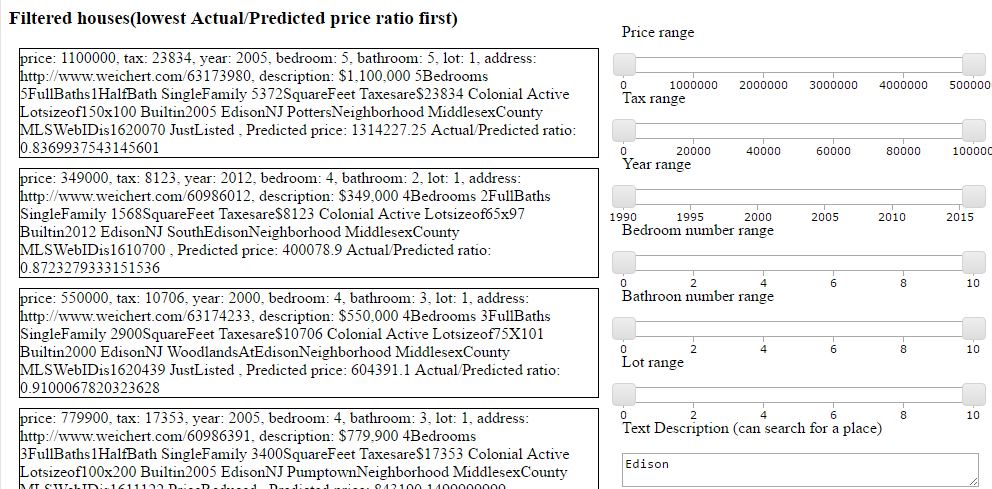
\includegraphics[width=0.5\textwidth]{houseedison.png}
\caption{}
\end{figure}

}
\item{}
	The error messages popping-up when users access and/or updates are denied (along with explanations and examples):
	\begin{itemize} 
	\item{The error message: There are no access denied error messages, because the data gathering/storing and the user interface are different parts in our application. The user interface has all access to data already scraped from the Web.}
	\item{The error message explanation (upon which violation it takes place): }
	The houses display being empty means that the request cannot be met within the current data set.
	\item{The error message example according to user(s) scenario(s): }
	If the user inputs a place name incorrectly (for example, type "Edison" as "Eddison") then most likely there will be no results displayed. What's more, since the result is updated in real time for every character of text, the user can notice the mistake immediately when he types "Edd". 
	 \end{itemize}
\item{}
	The information messages or results that pop-up in response to user interface events.
	\begin{itemize} 
	\item{The information message: }
	The "message" is the left side's houses display area being empty.
	\item{The information message explanation and the corresponding event trigger }
	Because the user starts typing "Edison" as "Eddison" in the text search box, the houses display becomes empty because "Edd" doesn't match any data records.
	\item{The error message example in response to data range constraints and the corresponding user's scenario }
	If the user inputs conditions that cannot be met, the displayed houses area will immediately be empty, and the user can simply correct it and do not need to click on a pop-up.
	The interface showing no houses match a mistake in input: 
	\begin{figure}
\centering
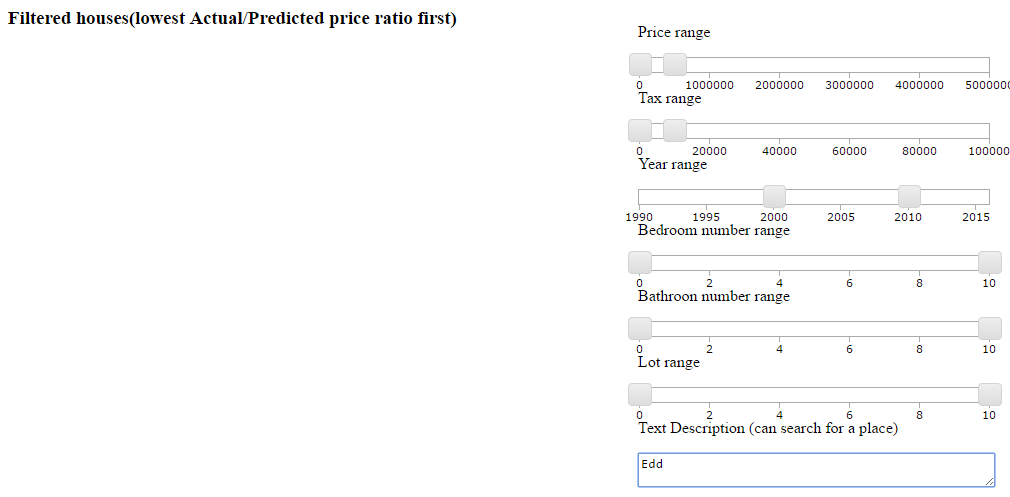
\includegraphics[width=0.5\textwidth]{housemistake.png}
\caption{}
\end{figure}
	 \end{itemize}
\item{}
	The  interface mechanisms that activate different views.
	\begin{itemize} 
	\item{The interface mechanism: }
	There is only one view, and the filtering of information is controlled by sliders and search boxes.
	 \end{itemize}

}
